%\documentclass[aspectratio=169,xcolor=dvipsnames]{beamer}
\documentclass[12pt]{beamer}
\usepackage[utf8]{inputenc}
\usepackage[english]{babel}
\usepackage[backend=bibtex]{biblatex}
\addbibresource{Project.bib}
\usetheme{AnnArbor}
\setbeamercolor{normal text}{bg=black!10}
\setbeamertemplate{caption}[numbered]
\begin{document}
\title{ELMA: Encrypted Offloading for Embedded NLP Applications}
\subtitle{Final Project Proposal}
\author[Group 3]{Group 3\\[\baselineskip]Yihua Liu, Shuocheng Chen, Yiming Ju}
\institute{UM-SJTU Joint Institute}
\date{\today}
\begin{frame}
    \titlepage
\end{frame}
\section{Objective}
\begin{frame}{Objectives}
    \begin{block}{An architecture}
        \begin{itemize}
            \item High-performance NLP model
            \item Restricted computational resources
            \item On embedded device
        \end{itemize}
    \end{block}
\end{frame}
\section{Overview}
\subsection{NLP}
\begin{frame}{NLP}
    \begin{block}{Definition}
        \begin{itemize}
            \item Natural Language Processing
            \item Focus on the theories and methods of effective communication between human and computer in the field of natural language.
        \end{itemize}
        
        
    \end{block}
    
    \begin{block}{Applications}
        \begin{itemize}
            \item Text classification
            \item Auto correct
            \item Machine translation
            \item Speech recognition
            \item ...
        \end{itemize}
    \end{block}

\end{frame}

\subsection{Computation offloading}
\begin{frame}{Computation offloading}
    \begin{block}{Definition}
        Migrate part of the data processing in the cloud to the local terminal devices.
    \end{block}
    \begin{block}{Advantages}
        \begin{itemize}
            \item Accelerate computation
            \item Save energy
            \item Lower latency
            \item Protect privacy
        \end{itemize}
    \end{block}
\end{frame}

\begin{frame}{Gantt Chart}
    \begin{figure}[!htb]
        \centering
        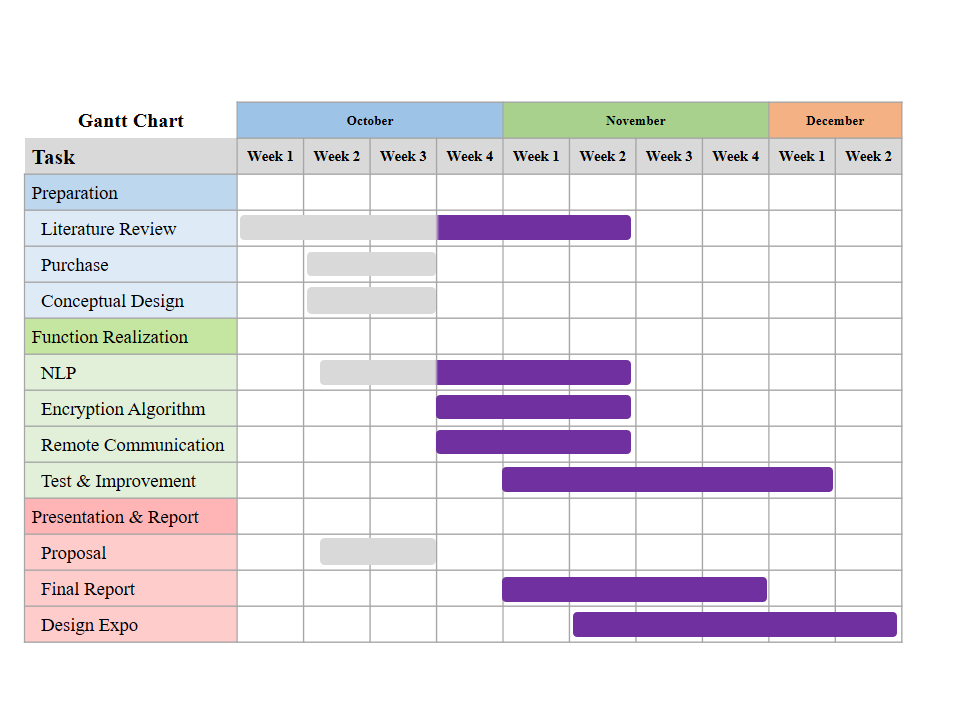
\includegraphics[width=0.8\textwidth]{Gantt Chart.png}
    \end{figure}
\end{frame}


\section{Concept Design}
\begin{frame}{Concept Design}
\begin{figure}[H]
    \centering
    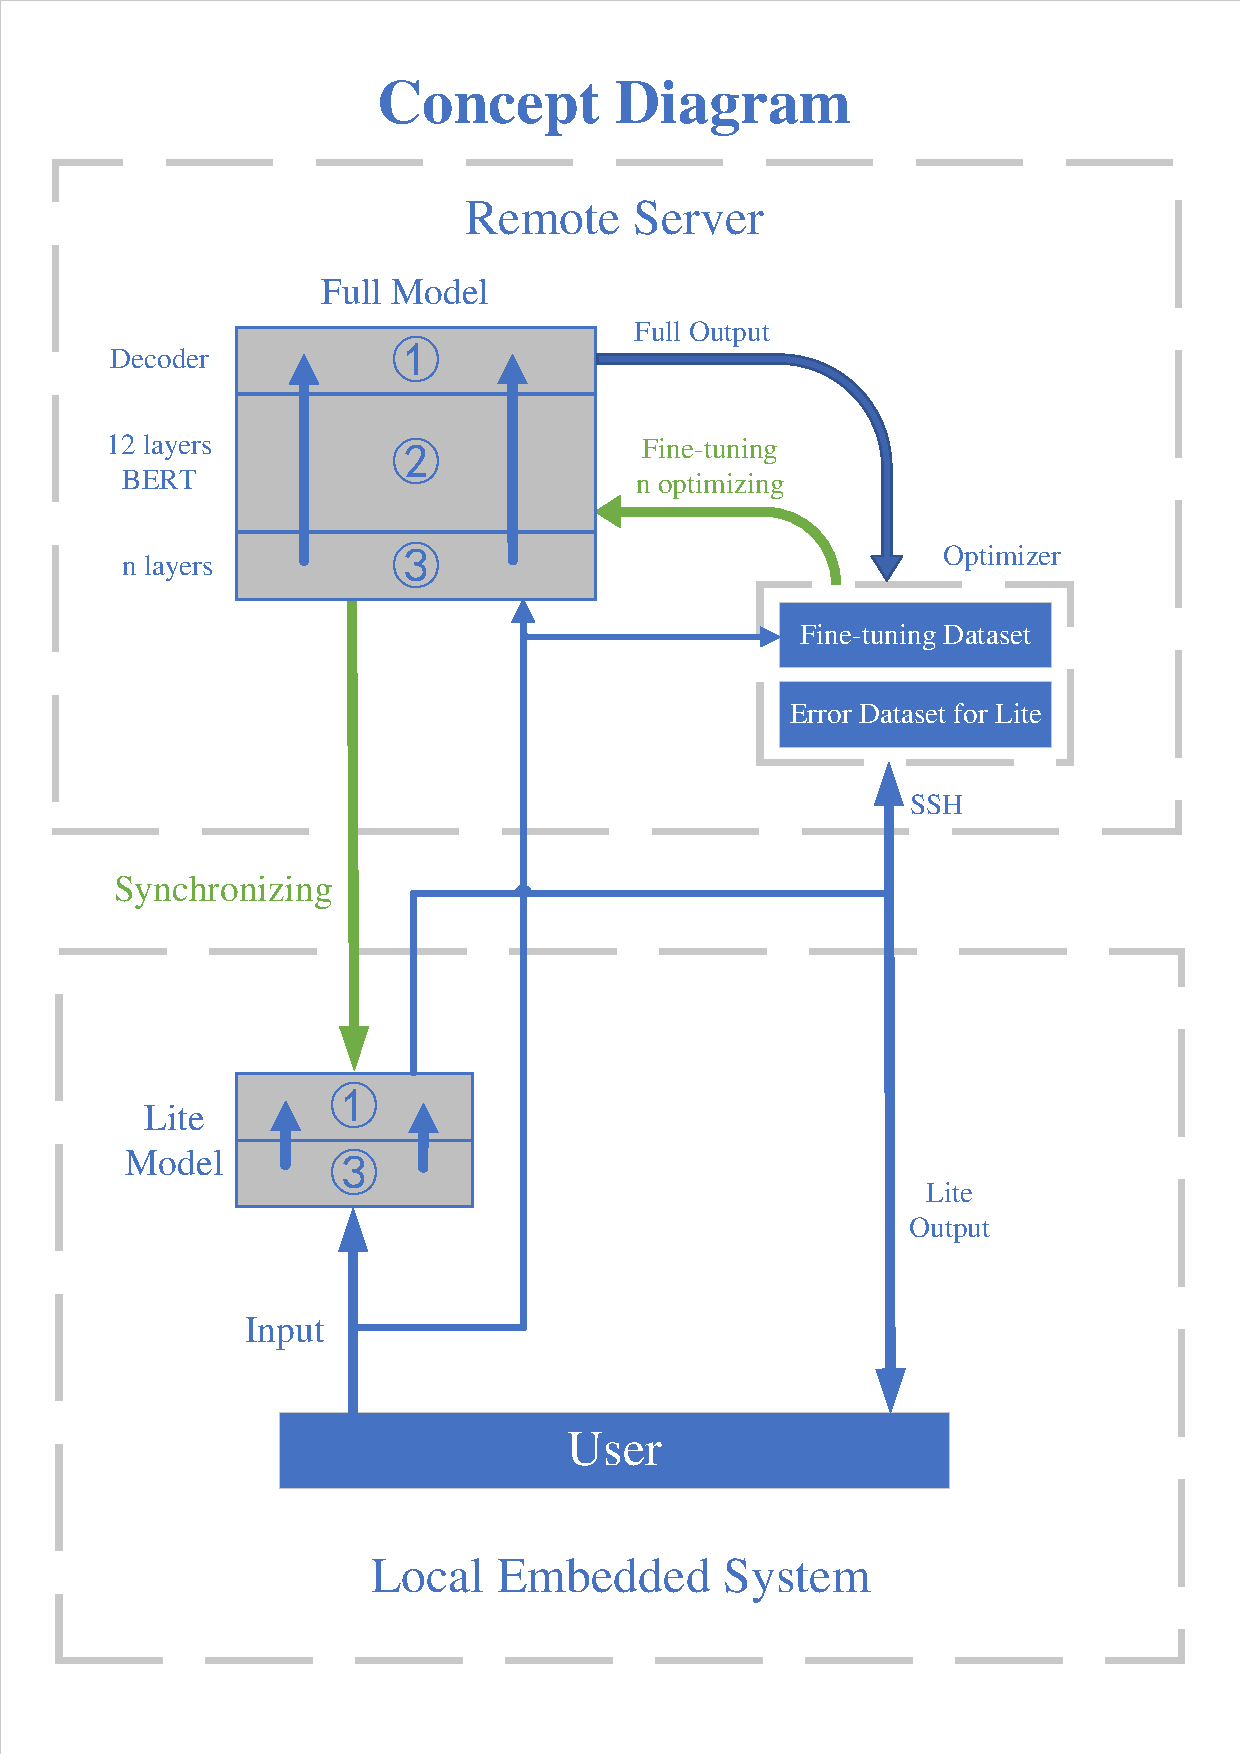
\includegraphics[width=0.45\textwidth]{Concept_Design.pdf}
    % \caption{Concept Design.}
\end{figure}
\end{frame}



\subsection{Transfer Learning}
\begin{frame}{Transfer Learning}
    \begin{block}{Methodology}
        \begin{itemize}
            \item Feature Extraction
            \item Fine-tuning
        \end{itemize}
    \end{block}
    
    \begin{block}{Benefits}
        \begin{itemize}
            \item simplification of task completion
            \item better performance
            \item computational redistribution
            \item edge computing
            \item ...
        \end{itemize}
    \end{block}
\end{frame}

\subsection{Transfer Learning}
\begin{frame}{BERT: Pre-trained State-of-the-Art Model}
    \begin{block}{Features}
        \begin{itemize}
            \item Fine-tuning based
            \item Universality for multiple tasks
        \end{itemize}
    \end{block}
    
    \begin{block}{Further Research}
        \begin{itemize}
            \item ALBERT: a lite BERT
            \item EdgeBERT
            \item Robust multi-tasking fine-tuning for BERT
            \item Few-sample fine-tuning optimization
            \item ...
        \end{itemize}
    \end{block}
\end{frame}


\subsection{Question Answering}
\begin{frame}{Question Answering}
    \begin{block}{Definition}
        Question answering programs can construct answers through the query of a knowledge base or an unstructured collection of documents in a natural language.
    \end{block}
    \begin{block}{Logical blocks}
        \begin{itemize}
            \item Data source
            \item Information retrieval system 
            \item Machine reading comprehension model
        \end{itemize}
    \end{block}
\end{frame}

\begin{frame}{Question Answering Example}
    \begin{block}{Text}
        The UM-SJTU Joint Institute has \textcolor{red}{more than 100} talented and dedicated faculty and staff members working to pursue its mission. We place a high priority on creating an environment that enables faculty and staff to do their best work and values the contributions of all employees in making the JI a world-class educational and research insitute in \textcolor{red}{China}. Employee commitment is vital to our success. Once JIer, JIer forever.
    \end{block}
    \begin{block}{Question}
        \begin{itemize}
            \item How many faculty in UM-SJTU?
            \item Where is JI?
        \end{itemize}
    \end{block}
    \url{https://visbert.demo.datexis.com/}
\end{frame}

\section{Concept Design}
\begin{frame}{Concept Design}
\begin{figure}[H]
    \centering
    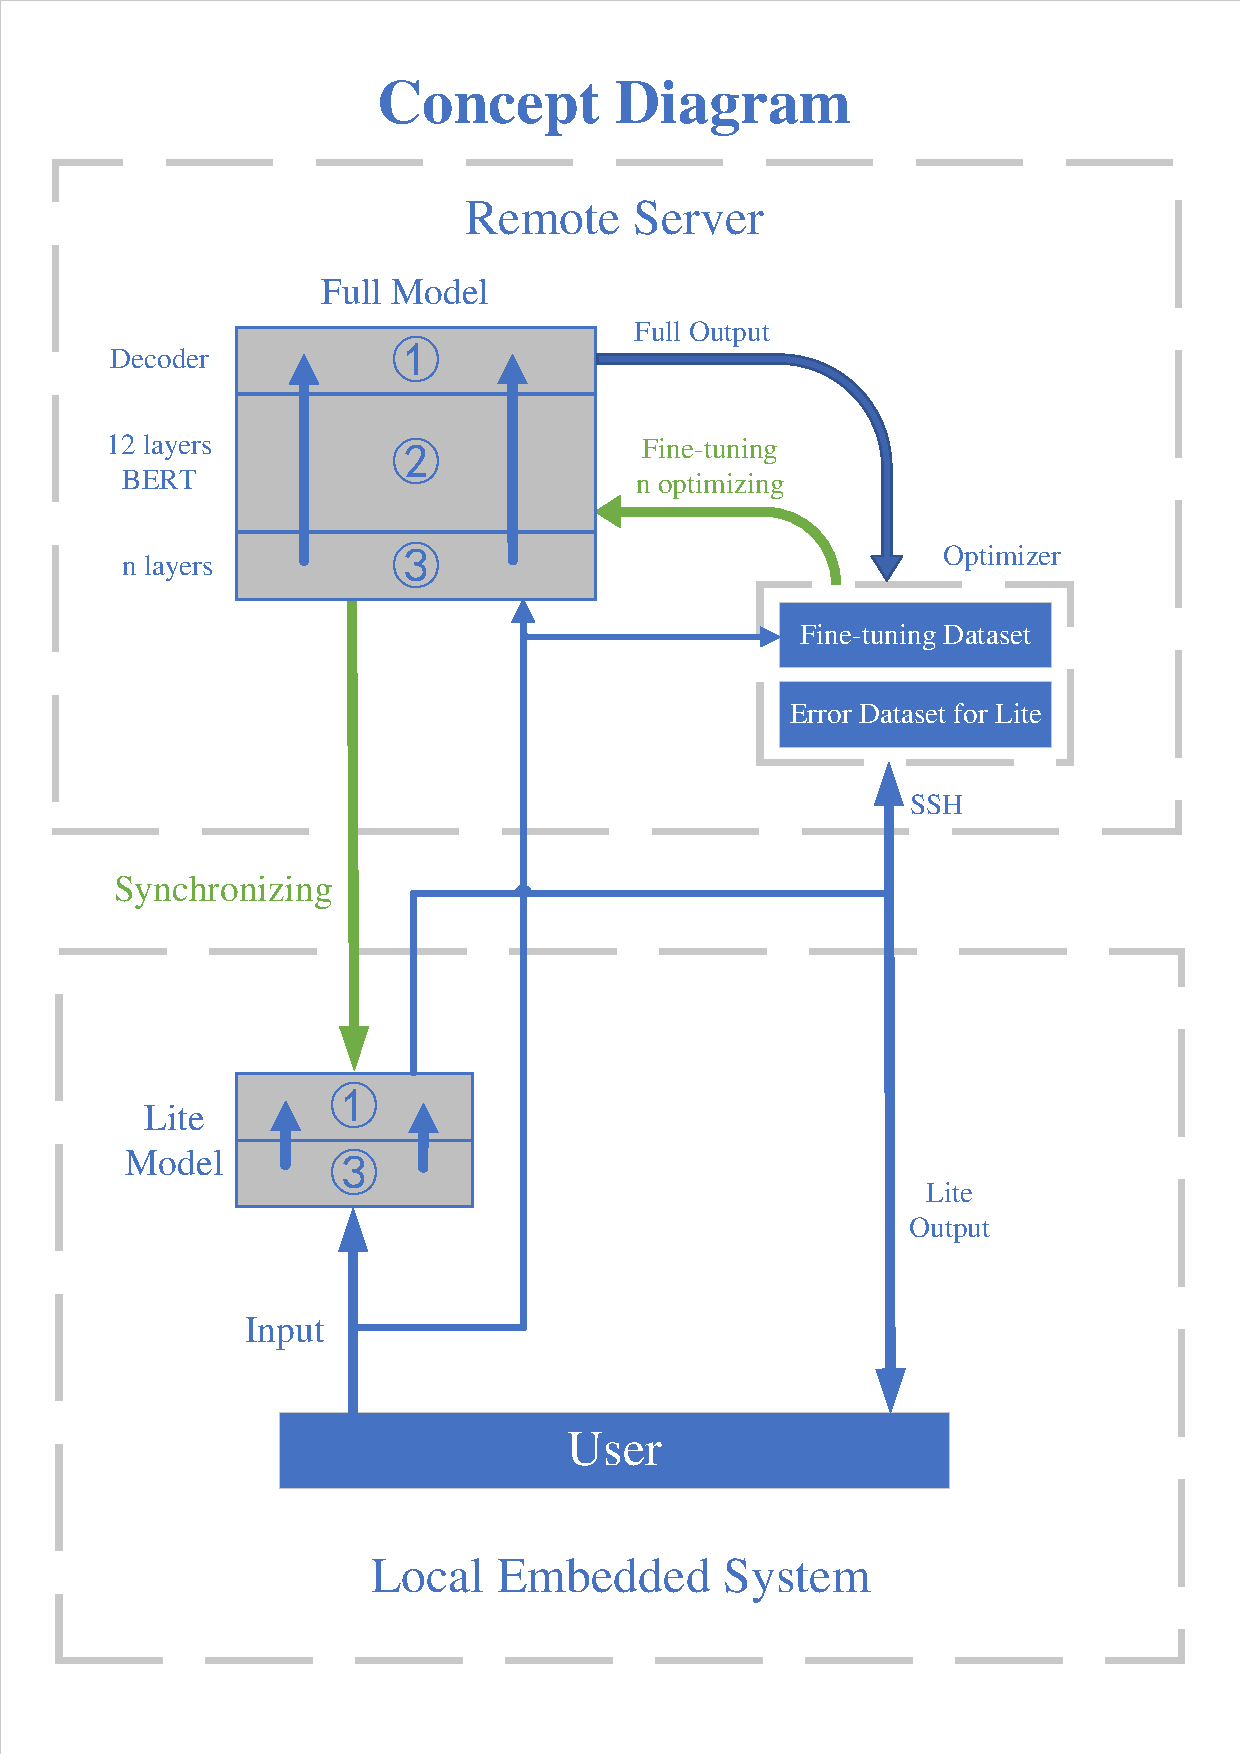
\includegraphics[width=0.45\textwidth]{Concept_Design.pdf}
    % \caption{Concept Design.}
\end{figure}
\end{frame}



\section{Related Work}
\begin{frame}{Related Work}{BERT: Bidirectional Encoder Representations from Transformers}
\begin{figure}[H]
    \centering
    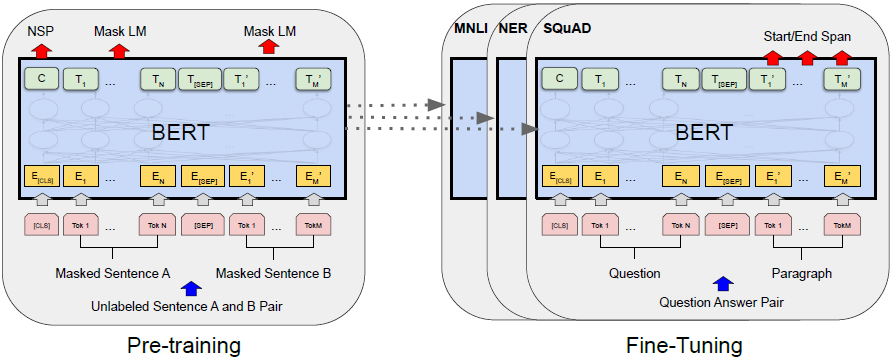
\includegraphics[width=0.5\textwidth]{BERT.png}
\end{figure}
\small The Bidirectional Encoder Representations from Transformers (BERT) \cite{devlin2019bert} divides the NLP model into two steps: pre-training and fine-tuning. The transformer encoder is with Gaussian Error Linear Units (GELU) nonlinearities. BERT uses a Masked Language Model (MLM) for language model pre-training and a Next Sentence Prediction (NSP) task for text-pair representation pre-training. For fine-tuning, take question answering applications as an example, BERT takes question-passage pairs as input and feeds token and \textsf{[CLS]} representations to output layers.
\end{frame}
\begin{frame}{Related Work}{ALBERT: A Lite BERT}
\begin{figure}[H]
    \centering
    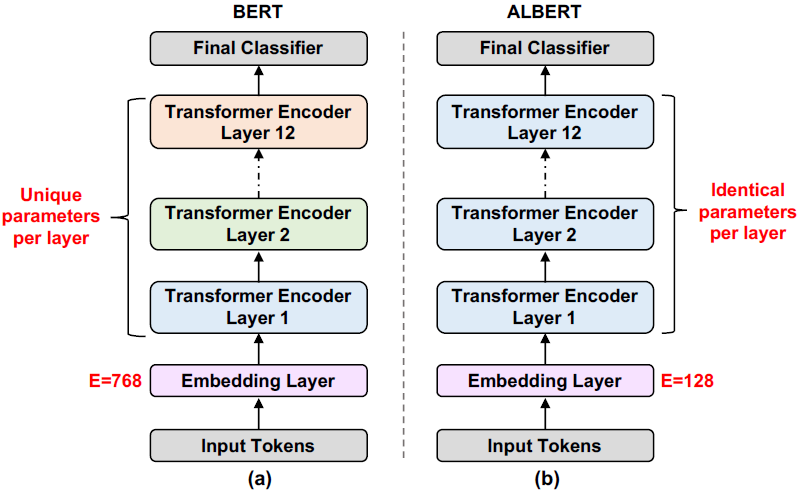
\includegraphics[width=0.5\textwidth]{ALBERT.png}
\end{figure}
\footnotesize ALBERT \cite{lan2020albert} does 3 significant improvements on traditional BERT model: factorized embedded parameterization, cross-layer parameter sharing, and inter-sentence coherence loss (sentence-order prediction (SOP) loss). ALBERT achieves better performance than BERT given larger configurations and fewer parameters. There are different methods to do cross-layer parameter sharing. ALBERT shares all parameters across layers, but parameters to share can be customized, such as feed-forward network (FFN) or attention parameters only.
\end{frame}
\begin{frame}{Related Work}{EdgeBERT}
\begin{figure}[H]
    \centering
    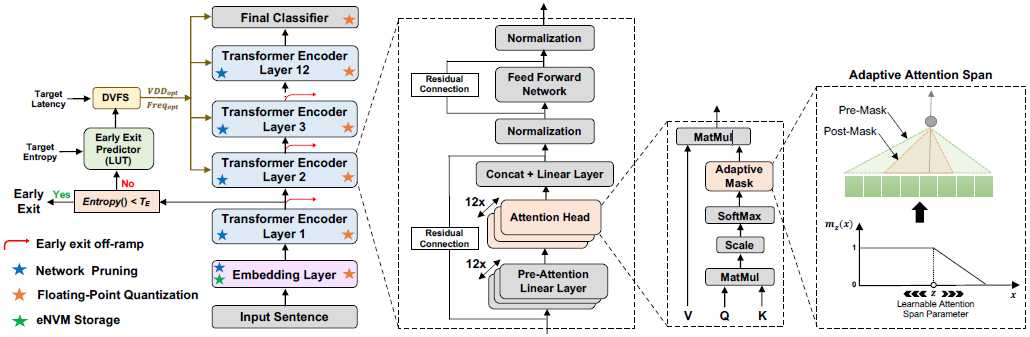
\includegraphics[width=0.8\textwidth]{EdgeBERT.png}
\end{figure}
\small EdgeBERT \cite{tambe2021edgebert} is a HW/SW (more specifically, hardware/algorithm) co-design for multi-task NLP whose purpose is to reduce energy consumption as much as possible while achieving improvements of accuracy and speed. EdgeBERT proposes several main improvents, including entropy-based early exit (EE) and dynamic voltage-frequency scaling (DVFS). Our work is inspired by the strategies that EdgeBERT adopts to save energy, which is very important for embedded systems.
\end{frame}

\section{Reference}
\begin{frame}{Reference}
    \printbibliography
\end{frame}

\section{Q \& A}
\begin{frame}
    \begin{center}
        Q \& A
    \end{center}
\end{frame}

\section{}
\begin{frame}
    \begin{center}
        Thanks!
    \end{center}
\end{frame}

\end{document}
